\subsection{Comunicazione con server}
\FloatBarrier
Utilizzando GWT-RPC, i nostri oggetti del modello vengono automaticamente serializzati quando vengono utilizzati come parametri per una chiamata RPC. Le uniche restrizioni sono date dall’obbligatorietà di implementare 
l’interfaccia \emph{Serializable} e dalla presenza di un costruttore senza argomenti. 

\begin{figure}[!htb]
\centering%
\includegraphics[scale=0.5]{AnatomySVG.png}%
\caption{GWT-RPC }\label{fig:GWT-RPC}%
\end{figure}
\FloatBarrier
Il primo passo per l’attuazione del servizio RPC è quello di dichiarare l’interfaccia di servizio che estenda l’interfaccia \emph{RemoteService} ed elenchi tutti i metodi RPC.
Successivamente definire una classe per implementare il codice server-side che estenda la classe \emph{RemoteServiceServlet} ed implementi l’interfaccia creata precedentemente. 
Non rimane che implementare la versione asincrona dell'interfaccia per l’applicazione client poiché ogni metodo chiamato deve essere asincrono.

\begin{figure}[!htb]
\centering%
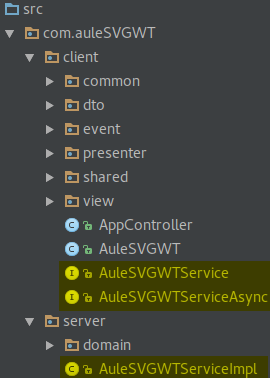
\includegraphics[scale=0.55]{rpcPack.png}%
\caption{Classi utilizzate per il servizio RPC. }\label{fig:RPCPack}%
\end{figure}